\chapter{Proposed Method}
\label{chap:proposed_method}

This chapter presents the proposed control framework for target-driven humanoid parkour in detail. The framework integrates five key components---a temporal-subsampled depth perception module, a GRU-based memory module, a cross-attention module, a mixture-of-experts (MoE) action head, and an adversarial motion prior (AMP) module---into a unified policy architecture that enables a humanoid robot to navigate complex obstacle-laden environments with natural, adaptive locomotion. We describe each component in terms of its design motivation, network architecture, and qualitative behavioral effects, and compare the proposed design choices against existing approaches reviewed in Chapter~\ref{sec:rw_locomotion}. Implementation details including reward functions, environment configurations, and training procedures are provided at the end of this chapter.

%% ============================================================
\section{Overview}
\label{sec:method_overview}
%% ============================================================

The central challenge addressed by the proposed framework is enabling a humanoid robot to perform target-driven parkour---navigating toward a sequence of goal positions across diverse, obstacle-rich terrain---using only onboard proprioceptive and depth-camera observations. This challenge demands three capabilities that existing methods fail to provide simultaneously: (1)~rich temporal-spatial terrain understanding from depth images, (2)~long-horizon terrain memory that persists across control steps, and (3)~adaptive skill selection for diverse terrain types.

Existing perceptive locomotion methods typically rely on one of two terrain representations: height scanners that cast rays downward to produce a one-dimensional height profile~\cite{zhang2024rpl,cheng2024extremeparkour}, or single-frame depth images processed through a convolutional encoder~\cite{zhu2024hiking,zhuang2024humanoidparkour}. Height scanners provide geometrically precise but spatially limited information---they capture only the terrain directly beneath the robot and cannot represent vertical obstacles such as walls or overhangs. Single-frame depth images provide richer spatial coverage but lack temporal context: the policy cannot distinguish whether an obstacle is approaching or receding, nor can it accumulate terrain information over time. Both representations suffer from a fundamental limitation---they treat terrain perception as a instantaneous snapshot rather than a temporal process, which is insufficient for parkour where the robot must anticipate upcoming obstacles and remember terrain features it has already traversed.

The proposed framework addresses these limitations through the architecture illustrated in Figure~\ref{fig:overall_architecture}. The policy receives two categories of observations: proprioceptive observations (joint positions, velocities, base orientation, and velocity commands) and depth image observations from an onboard camera. These observations are processed by a \emph{Memory-Attention Encoder} that produces four output streams: (1)~a memory latent vector from a GRU-based recurrent module, (2)~an attention latent vector from a cross-attention module, (3)~a depth latent vector from a convolutional encoder, and (4)~the raw proprioceptive observations. These four streams are concatenated and fed into a Mixture-of-Experts (MoE) actor-critic network, which outputs joint position targets. The entire policy is trained with PPO augmented by an AMP discriminator that encourages natural, human-like motion style.

\begin{figure}[t]
    \centering
    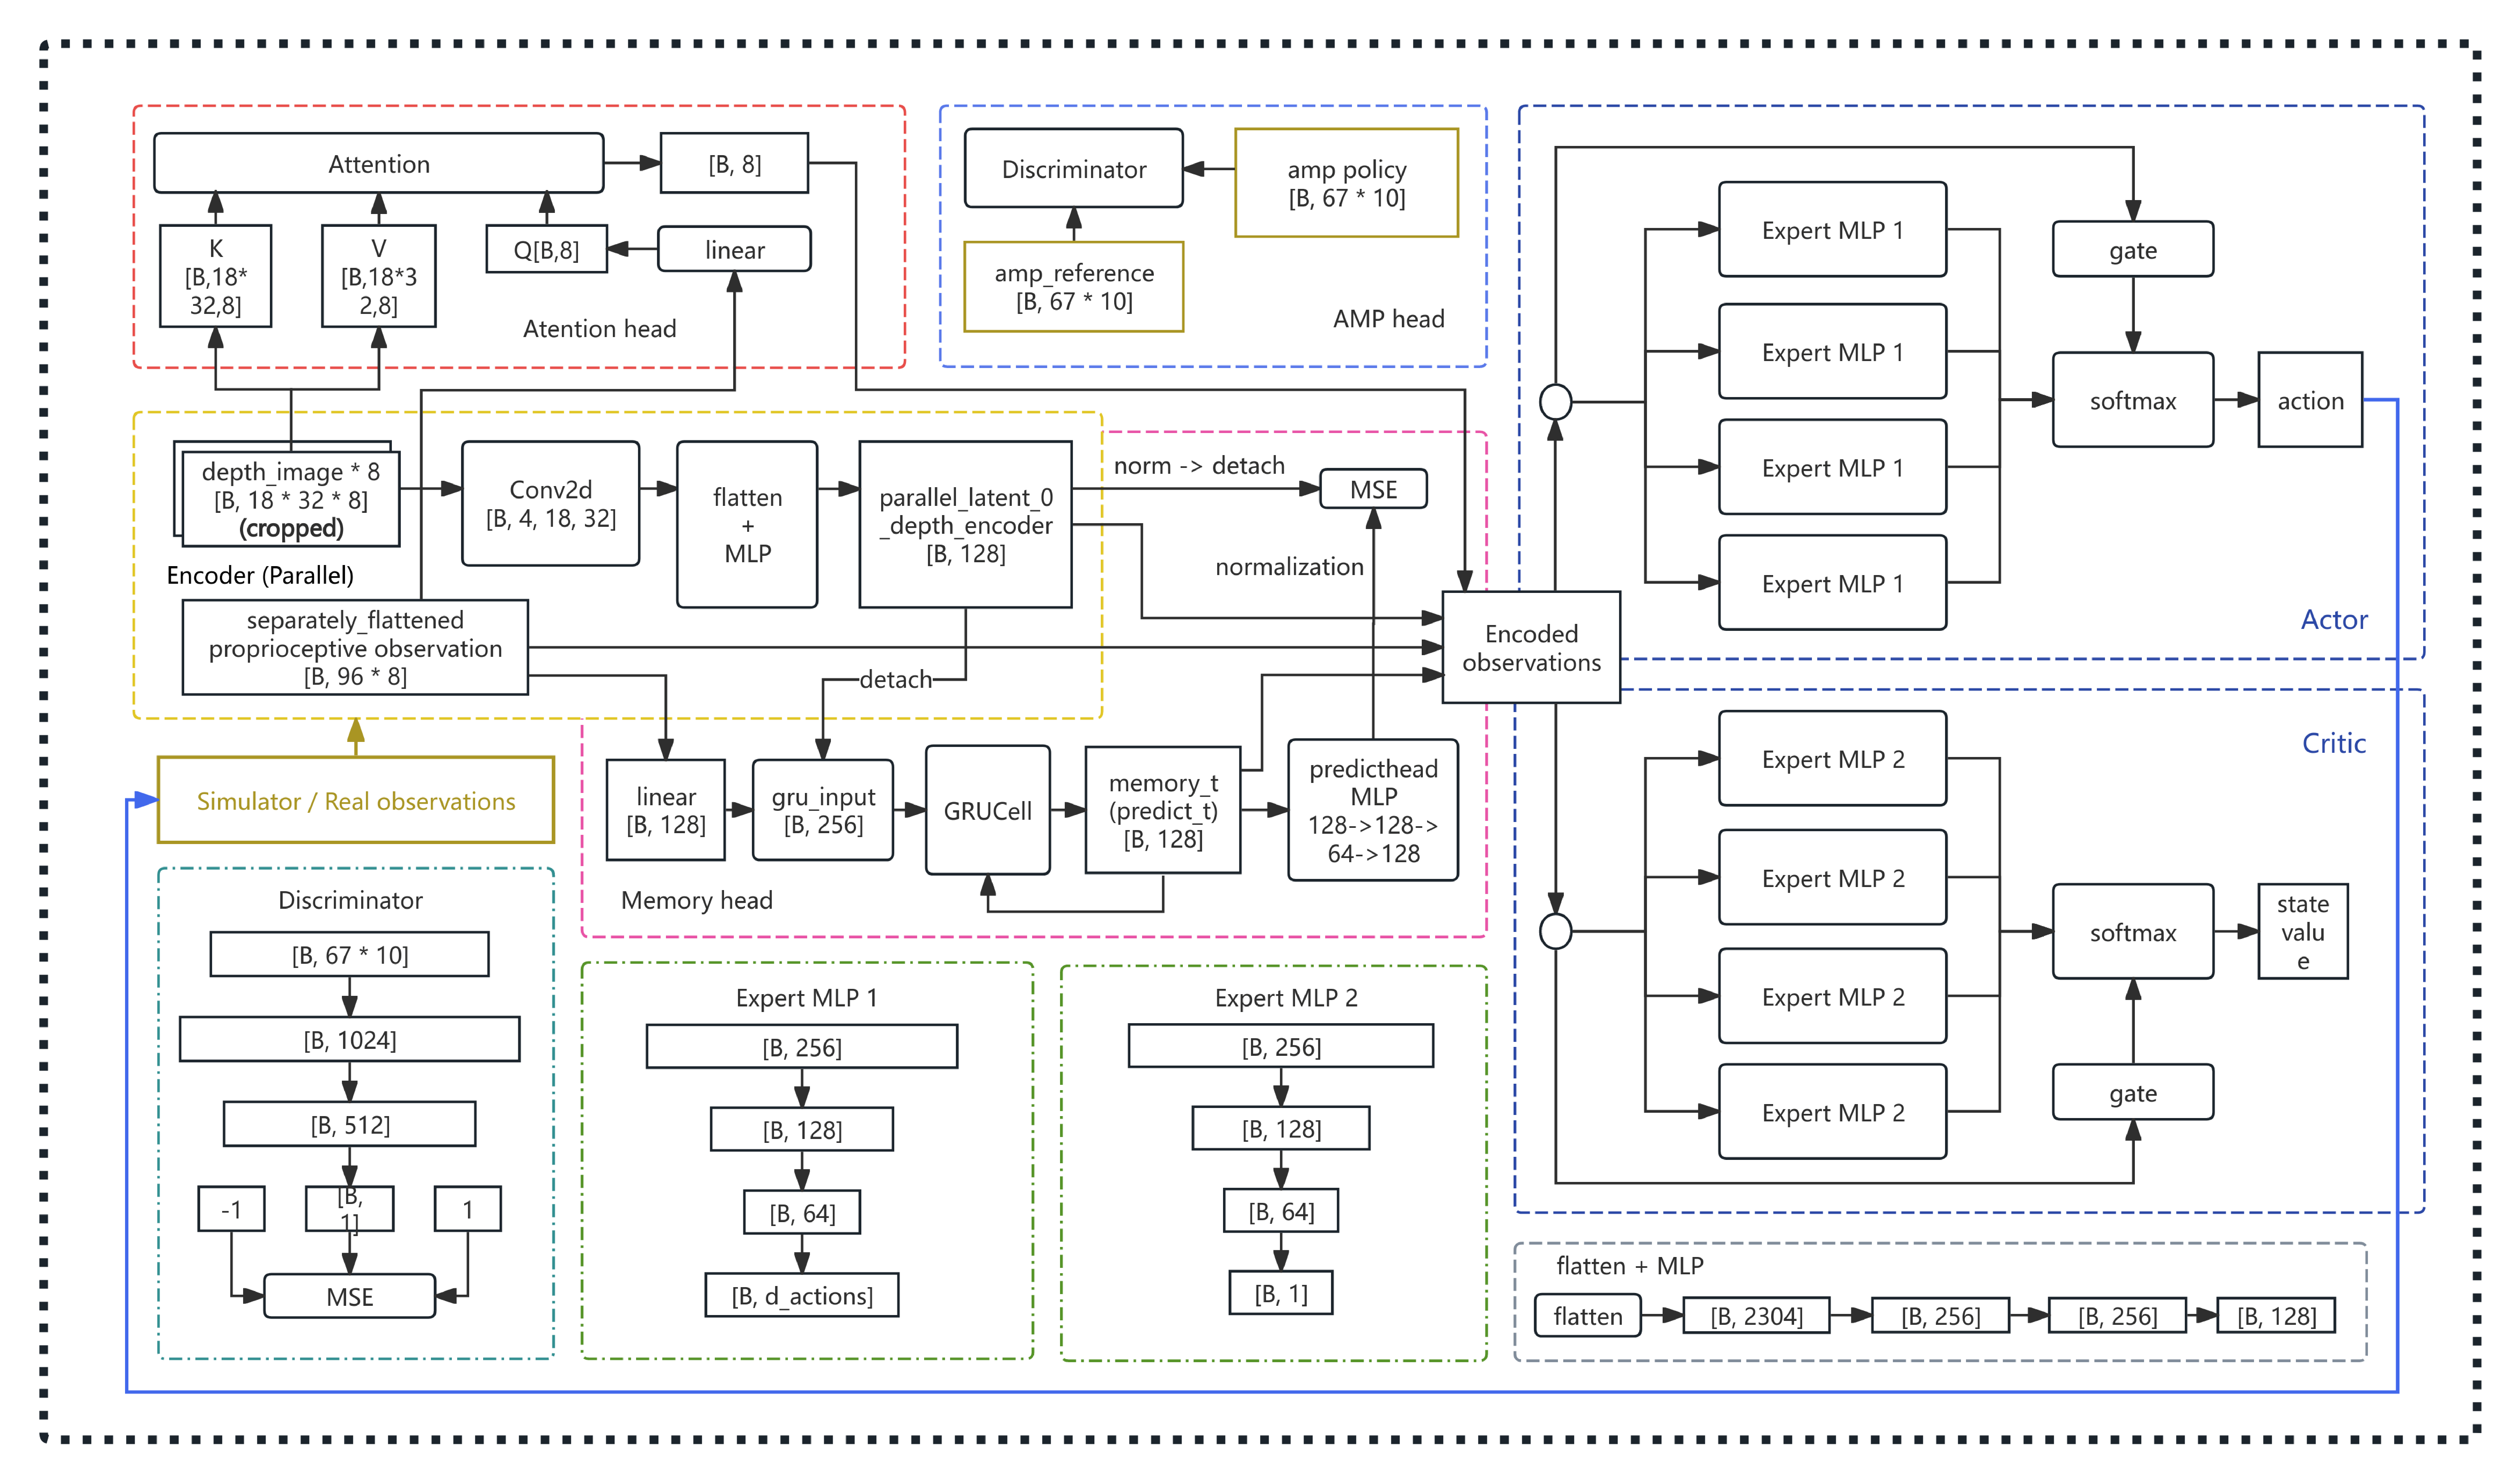
\includegraphics[width=\textwidth]{figures/ch3_overall_architecture.pdf}
    \caption{Overall architecture of the proposed framework. Proprioceptive observations and temporal-subsampled depth images are processed by the Memory-Attention Encoder, which produces four output streams: memory latent $\mathbf{m}_t$, attention latent $\mathbf{a}_t$, depth latent $\mathbf{z}_t^d$, and raw proprioceptive observations $\mathbf{o}_t^{\text{prop}}$. These are concatenated and fed into the MoE actor-critic, which outputs joint position targets. The AMP discriminator provides an adversarial style reward. The memory hidden state $\mathbf{h}_t$ is maintained across time steps and reset at episode boundaries.}
    \label{fig:overall_architecture}
\end{figure}

The key innovations of the proposed architecture are:

\begin{enumerate}
    \item \textbf{Temporal-subsampled depth image stack.} Rather than processing consecutive depth frames or a single frame, the proposed method samples depth images at fixed intervals (every 5 control steps) and stacks 8 sampled frames into a single multi-channel input. This design embeds temporal information into the spatial structure of the depth representation, allowing the convolutional encoder and attention module to jointly reason about spatial and temporal terrain features.

    \item \textbf{GRU memory with consistency loss.} A GRU cell maintains a hidden state that accumulates terrain information over time, enabling the policy to remember terrain features beyond the limited temporal window of the depth stack. A novel consistency loss ensures that the memory representation encodes meaningful terrain information by requiring the memory output to predict the current depth latent.

    \item \textbf{Cross-attention for spatial focus.} A multi-head cross-attention mechanism allows the policy to selectively focus on the most task-relevant regions of the depth image, using the robot's current proprioceptive state as a query. This enables adaptive spatial attention---for example, focusing on nearby obstacles when approaching a gap, or attending to wall structures when navigating confined spaces.

    \item \textbf{Mixture-of-Experts for skill routing.} Multiple expert networks with a learned gating mechanism enable the policy to specialize different expert sub-networks for different terrain types and locomotion skills, without requiring explicit skill decomposition or a high-level skill selector.

    \item \textbf{Adversarial motion priors with self-collected data.} The AMP module is trained on motion capture data collected by the authors and retargeted to the robot's morphology, covering walking, running, and stair-climbing motions that are directly relevant to parkour scenarios.
\end{enumerate}

The interaction between these components creates a complementary system: the memory module provides long-horizon terrain understanding (addressing the temporal dimension), the attention module provides spatial selectivity (addressing the spatial dimension), the MoE module provides skill diversity, and the AMP module provides motion style regularization. The temporal-subsampled depth stack serves as the perceptual foundation that bridges the memory and attention modules by encoding both spatial and temporal terrain features in a unified representation.

%% ============================================================
\section{Policy Input Representation}
\label{sec:policy_input}
%% ============================================================

The design of the policy input representation is critical for parkour: the observations must provide sufficient information for the policy to perceive terrain geometry, track velocity commands, and maintain awareness of the robot's internal state, while remaining compatible with real-time inference on onboard hardware. This section describes the two primary observation categories---proprioceptive observations and depth image observations---as well as the target-driven command system that guides the robot through the parkour course.

\subsection{Proprioceptive Observations}
\label{sec:proprio_obs}

The proprioceptive observation group provides the policy with information about the robot's internal state and the commanded velocities. To enable the policy to infer velocity and acceleration from position history, each scalar observation is repeated over a history window of $H=8$ consecutive time steps and flattened into a single vector. The proprioceptive observation components are listed in Table~\ref{tab:proprio_obs}.

\begin{table}[t]
\centering
\caption{Proprioceptive observation components for the policy. Each component is repeated over a history window of $H=8$ time steps. Additive uniform noise is applied during training for robustness.}
\label{tab:proprio_obs}
\footnotesize
\begin{tabular}{@{}lp{5.5cm}ccc@{}}
\toprule
\textbf{Component} & \textbf{Description} & \textbf{Dim.} & \textbf{Noise Range} & \textbf{Scale} \\
\midrule
Base angular velocity & Angular velocity in body frame & 3 & $[-0.2, 0.2]$ & 0.25 \\
Projected gravity & Gravity vector in body frame & 3 & $[-0.05, 0.05]$ & --- \\
Velocity commands & Target linear \& angular velocities & 3 & --- & --- \\
Joint positions (relative) & Current joint pos.\ minus default pos. & 29 & $[-0.01, 0.01]$ & --- \\
Joint velocities (relative) & Joint velocities & 29 & $[-0.5, 0.5]$ & 0.05 \\
Last action & Previous step's action output & 29 & --- & --- \\
\midrule
\textbf{Total per step} & & \textbf{96} & & \\
\textbf{Total with history} & $96 \times H$ & \textbf{768} & & \\
\bottomrule
\end{tabular}
\end{table}

The base angular velocity and projected gravity observations provide the policy with information about the robot's orientation and rotational dynamics. The velocity commands encode the target motion specified by the command system (described in Section~\ref{sec:target_command}). Joint positions and velocities provide the policy with fine-grained information about the robot's current pose and motion, enabling precise foot placement and whole-body coordination. The last action is included to enable the policy to produce smooth, temporally consistent actions by conditioning the current action on the previous one.

Additive uniform noise is applied to the proprioceptive observations during training to improve robustness to sensor noise and calibration errors at deployment. The noise ranges are chosen to be larger than the expected sensor noise in simulation but smaller than the signal magnitude, ensuring that the policy learns to be robust without losing information.

For the critic network, an additional observation group is provided that includes the base linear velocity (3 dimensions, repeated over $H=8$ steps for a total of 24 additional dimensions). This privileged information is available to the critic during training but not to the actor at deployment, following the asymmetric actor-critic paradigm that has been shown to improve training efficiency in locomotion tasks~\cite{zhang2024rpl}.

\subsection{Depth Image Observations}
\label{sec:depth_obs}

The depth image observation is the primary source of exteroceptive information for the policy, providing a direct measurement of the terrain geometry in front of the robot. Unlike height scanners that cast rays downward to produce a one-dimensional height profile~\cite{zhang2024rpl,cheng2024extremeparkour}, depth cameras provide a two-dimensional image that captures both the horizontal and vertical structure of the terrain, including walls, overhangs, and obstacles at varying distances.

\subsubsection{Sensor Configuration}

The depth camera is mounted on the robot's torso link, providing a first-person perspective of the terrain ahead. The camera has a horizontal field of view (FOV) of $87.5^\circ$ and a vertical FOV of $58.3^\circ$, with a resolution of $64 \times 36$ pixels. The depth measurements are clipped to a maximum range and normalized to the range $[0, 1]$ based on a depth range of $[0, 2.5]$~m, with a minimum distance of $0.1$~m. The camera update period is $20$~ms, corresponding to the control frequency of the policy.

\subsubsection{Temporal-Subsampled Depth Image Stack}
\label{sec:temporal_subsample}

A key innovation of the proposed framework is the temporal-subsampled depth image stack. Rather than processing consecutive depth frames (which would provide redundant information due to the high frame rate relative to the control frequency) or a single frame (which would lack temporal context), the proposed method samples depth images at fixed intervals and stacks the sampled frames into a multi-channel input.

Specifically, the depth observation function maintains a history buffer of the most recent depth frames. Every $S=5$ control steps, one frame is sampled from the buffer and appended to the output stack. The output stack contains $F=8$ frames, covering a total temporal span of:
\begin{equation}
    T_{\text{coverage}} = S \times F \times \Delta t = 5 \times 8 \times 0.02 = 0.8~\text{s}
\end{equation}
where $\Delta t = 0.02$~s is the control period. This design embeds temporal information into the spatial structure of the depth representation: each of the 8 channels in the depth stack corresponds to a different time step, allowing the convolutional encoder and attention module to jointly reason about spatial and temporal terrain features.

\begin{figure}[t]
    \centering
    
\includegraphics[width=0.85\textwidth]{figures/ch3_temporal_subsample.pdf}
    \caption{Illustration of the temporal-subsampled depth image stack. Consecutive depth frames (top row) are sampled every $S=5$ steps, producing 8 frames that span approximately 0.8 seconds of terrain history. The sampled frames are stacked along the channel dimension to form the input to the depth encoder. Earlier frames (left) provide information about terrain the robot has already traversed, while later frames (right) provide information about upcoming terrain.}
    \label{fig:temporal_subsample}
\end{figure}

The motivation for this design arises from the observation that consecutive depth frames at the control frequency contain largely redundant information---the terrain does not change significantly between adjacent 20~ms steps. By subsampling at intervals of 5 steps, each frame in the stack captures a meaningfully different terrain state, providing the policy with a compact temporal summary of the terrain evolution. This is particularly important for parkour, where the robot must anticipate upcoming obstacles (e.g., a gap approaching from a distance) and remember terrain features it has already traversed (e.g., a step it has just climbed).

Compared to the height scanner representation used in RPL~\cite{zhang2024rpl} and Extreme Parkour~\cite{cheng2024extremeparkour}, the temporal-subsampled depth stack provides three advantages: (1)~it captures vertical terrain structure (walls, overhangs) that height scanners cannot represent; (2)~it provides temporal context through the multi-frame stack, enabling the policy to infer terrain dynamics; and (3)~it preserves the full 2D spatial structure of the depth image, enabling the attention module to perform spatially selective processing.

Compared to the single-frame depth processing used in Hiking in the Wild~\cite{zhu2024hiking} and Humanoid Parkour Learning~\cite{zhuang2024humanoidparkour}, the temporal-subsampled depth stack provides temporal context that single-frame processing cannot: the policy can observe how terrain features change across the 8 sampled frames, enabling it to distinguish between approaching and receding obstacles, estimate the speed of terrain changes, and accumulate information about the terrain ahead.

\subsubsection{Depth Noise Pipeline}

To bridge the sim-to-real gap in depth perception, a multi-stage noise pipeline is applied to the depth images during training:

\begin{enumerate}
    \item \textbf{Crop and Resize.} A rectangular region of the depth image is cropped (crop region: rows 18--34, columns 0--16, producing a $16 \times 16$ sub-image) and resized back to the original resolution. This simulates the limited field of view and resolution of real depth sensors.

    \item \textbf{Gaussian Blur.} A Gaussian blur with kernel size 3 and standard deviation $\sigma=1$ is applied to smooth the depth image, simulating the noise characteristics of real depth sensors that produce spatially correlated measurement errors.

    \item \textbf{Depth Normalization.} Raw depth values are normalized from the range $[0, 2.5]$~m to $[0, 1]$, providing a consistent input scale for the encoder regardless of the absolute depth range.
\end{enumerate}

Additionally, a random frame delay of 0--1 steps is applied to simulate the latency of real depth sensors, and additive Gaussian noise and depth artifact noise are applied during training for further robustness.

\subsection{Target-Driven Command System}
\label{sec:target_command}

The velocity commands that guide the robot through the parkour course are generated by a target-driven command system. Unlike fixed-velocity or random-velocity command systems used in previous locomotion work~\cite{rudin2016walk,margolis2024rapidlocomotion}, the proposed system computes velocity commands based on the direction and distance to a target position sampled on the terrain.

At the beginning of each episode and at regular resampling intervals, a target position is randomly sampled from a set of valid target positions on the terrain. The valid target positions are pre-computed flat patches on each sub-terrain, ensuring that the target is always reachable. The command system then computes:
\begin{equation}
    \mathbf{c}_t^{\text{vel}} = \begin{bmatrix} k_v \cdot \Delta x_t^b \\ k_v \cdot \Delta y_t^b \\ k_h \cdot \Delta \psi_t \end{bmatrix}
\end{equation}
where $\Delta x_t^b$ and $\Delta y_t^b$ are the target position coordinates in the robot's body frame, $\Delta \psi_t$ is the heading error to the target, and $k_v = 2.0$ and $k_h = 2.0$ are the velocity and heading control stiffness gains, respectively. The velocity commands are clamped to terrain-specific ranges (e.g., forward velocity $v_x \in [0.45, 1.0]$~m/s for rough terrain, $v_x \in [0.3, 0.8]$~m/s for stair terrain).

When the robot is within a threshold distance of the target ($d_t < 0.4$~m), the velocity commands are set to zero, indicating that the current target has been reached. A proportion of environments are designated as ``standing'' environments where the velocity commands are always zero, encouraging the policy to learn stable standing behavior.

This target-driven command system provides a natural curriculum for parkour learning: the robot must navigate toward specific goal positions across diverse terrain, requiring it to develop terrain-appropriate locomotion strategies (e.g., stepping carefully on stairs, leaping across gaps, slowing down near walls) rather than simply moving at a fixed speed.

%% ============================================================
\section{Memory Module}
\label{sec:memory_module}
%% ============================================================

\subsection{Motivation}

Parkour locomotion requires the policy to maintain a persistent understanding of the terrain beyond the limited temporal window of the depth image stack. While the temporal-subsampled depth stack (Section~\ref{sec:temporal_subsample}) provides terrain information spanning approximately 0.8 seconds, many parkour scenarios demand longer-horizon terrain memory: the robot must remember that it has just climbed a step (to adjust its posture accordingly), recall the location of a gap it observed several seconds ago (to plan its approach), or maintain awareness of the overall terrain profile (to select appropriate locomotion strategies).

Existing approaches to memory in locomotion policies rely primarily on recurrent neural networks (RNNs) with implicit hidden states. DreamWaQ~\cite{nahraendra2024dreamwaq} uses an RNN hidden state as an implicit terrain imagination, but this representation is not explicitly supervised and may not encode terrain information in a structured or interpretable manner. LocoFormer~\cite{liu2024locoformer} uses a Transformer architecture with self-attention over observation sequences, but the quadratic complexity of self-attention limits the sequence length that can be processed in real time. Neither approach provides an explicit mechanism to ensure that the memory representation encodes meaningful terrain information.

The proposed memory module addresses these limitations through two design choices: (1)~a GRU cell that maintains a compact hidden state updated at each time step, providing a fixed-cost recurrent memory that can persist information over arbitrarily long horizons; and (2)~a consistency loss that explicitly supervises the memory representation to encode terrain information relevant to the current observation, ensuring that the memory state carries meaningful semantic content rather than degenerating into an uninterpretable latent code.

\subsection{Network Architecture}

The memory module operates on two inputs: the raw proprioceptive observations $\mathbf{o}_t^{\text{prop}}$ and the depth latent $\mathbf{z}_t^d$ produced by the depth encoder (described in Section~\ref{sec:depth_obs}). The architecture is as follows:

\begin{enumerate}
    \item \textbf{State projection.} The proprioceptive observations are projected through a linear layer:
    \begin{equation}
        \mathbf{s}_t = W_s \mathbf{o}_t^{\text{prop}} + \mathbf{b}_s, \quad \mathbf{s}_t \in \mathbb{R}^{128}
    \end{equation}
    where $W_s \in \mathbb{R}^{128 \times d_{\text{prop}}}$ and $\mathbf{b}_s \in \mathbb{R}^{128}$ are learnable parameters.

    \item \textbf{Input concatenation.} The projected state is concatenated with the \emph{detached} depth latent:
    \begin{equation}
        \mathbf{x}_t^{\text{mem}} = [\mathbf{s}_t \, \| \, \text{sg}(\mathbf{z}_t^d)], \quad \mathbf{x}_t^{\text{mem}} \in \mathbb{R}^{256}
    \end{equation}
    where $\text{sg}(\cdot)$ denotes the stop-gradient operator that prevents gradients from flowing through the depth latent into the memory input. This detachment is critical: it ensures that the memory module does not interfere with the depth encoder's training signal, allowing the two modules to be trained independently while still providing the memory with terrain information.

    \item \textbf{GRU update.} The concatenated input is fed into a GRU cell that updates the memory hidden state:
    \begin{equation}
        \mathbf{h}_t = \text{GRUCell}(\mathbf{x}_t^{\text{mem}}, \mathbf{h}_{t-1}), \quad \mathbf{h}_t \in \mathbb{R}^{128}
    \end{equation}
    The GRU cell uses gated updates with reset and update gates to selectively incorporate new information and retain relevant past information. The hidden size of 128 provides a compact representation that is sufficient for encoding terrain features while remaining computationally efficient for real-time inference.

    \item \textbf{Memory output.} The updated hidden state $\mathbf{h}_t$ serves as the memory latent $\mathbf{m}_t = \mathbf{h}_t$, which is concatenated with the other encoder outputs and fed into the MoE actor-critic.
\end{enumerate}

The memory hidden state is maintained across time steps during both training and inference. At episode boundaries (when a done signal is received), the hidden state is reset to zero for the corresponding environments. During training, the hidden states are stored in the rollout buffer and passed to the encoder during the policy update phase, enabling proper backpropagation through time (BPTT) across the stored trajectory segments.

\begin{figure}[t]
    \centering
    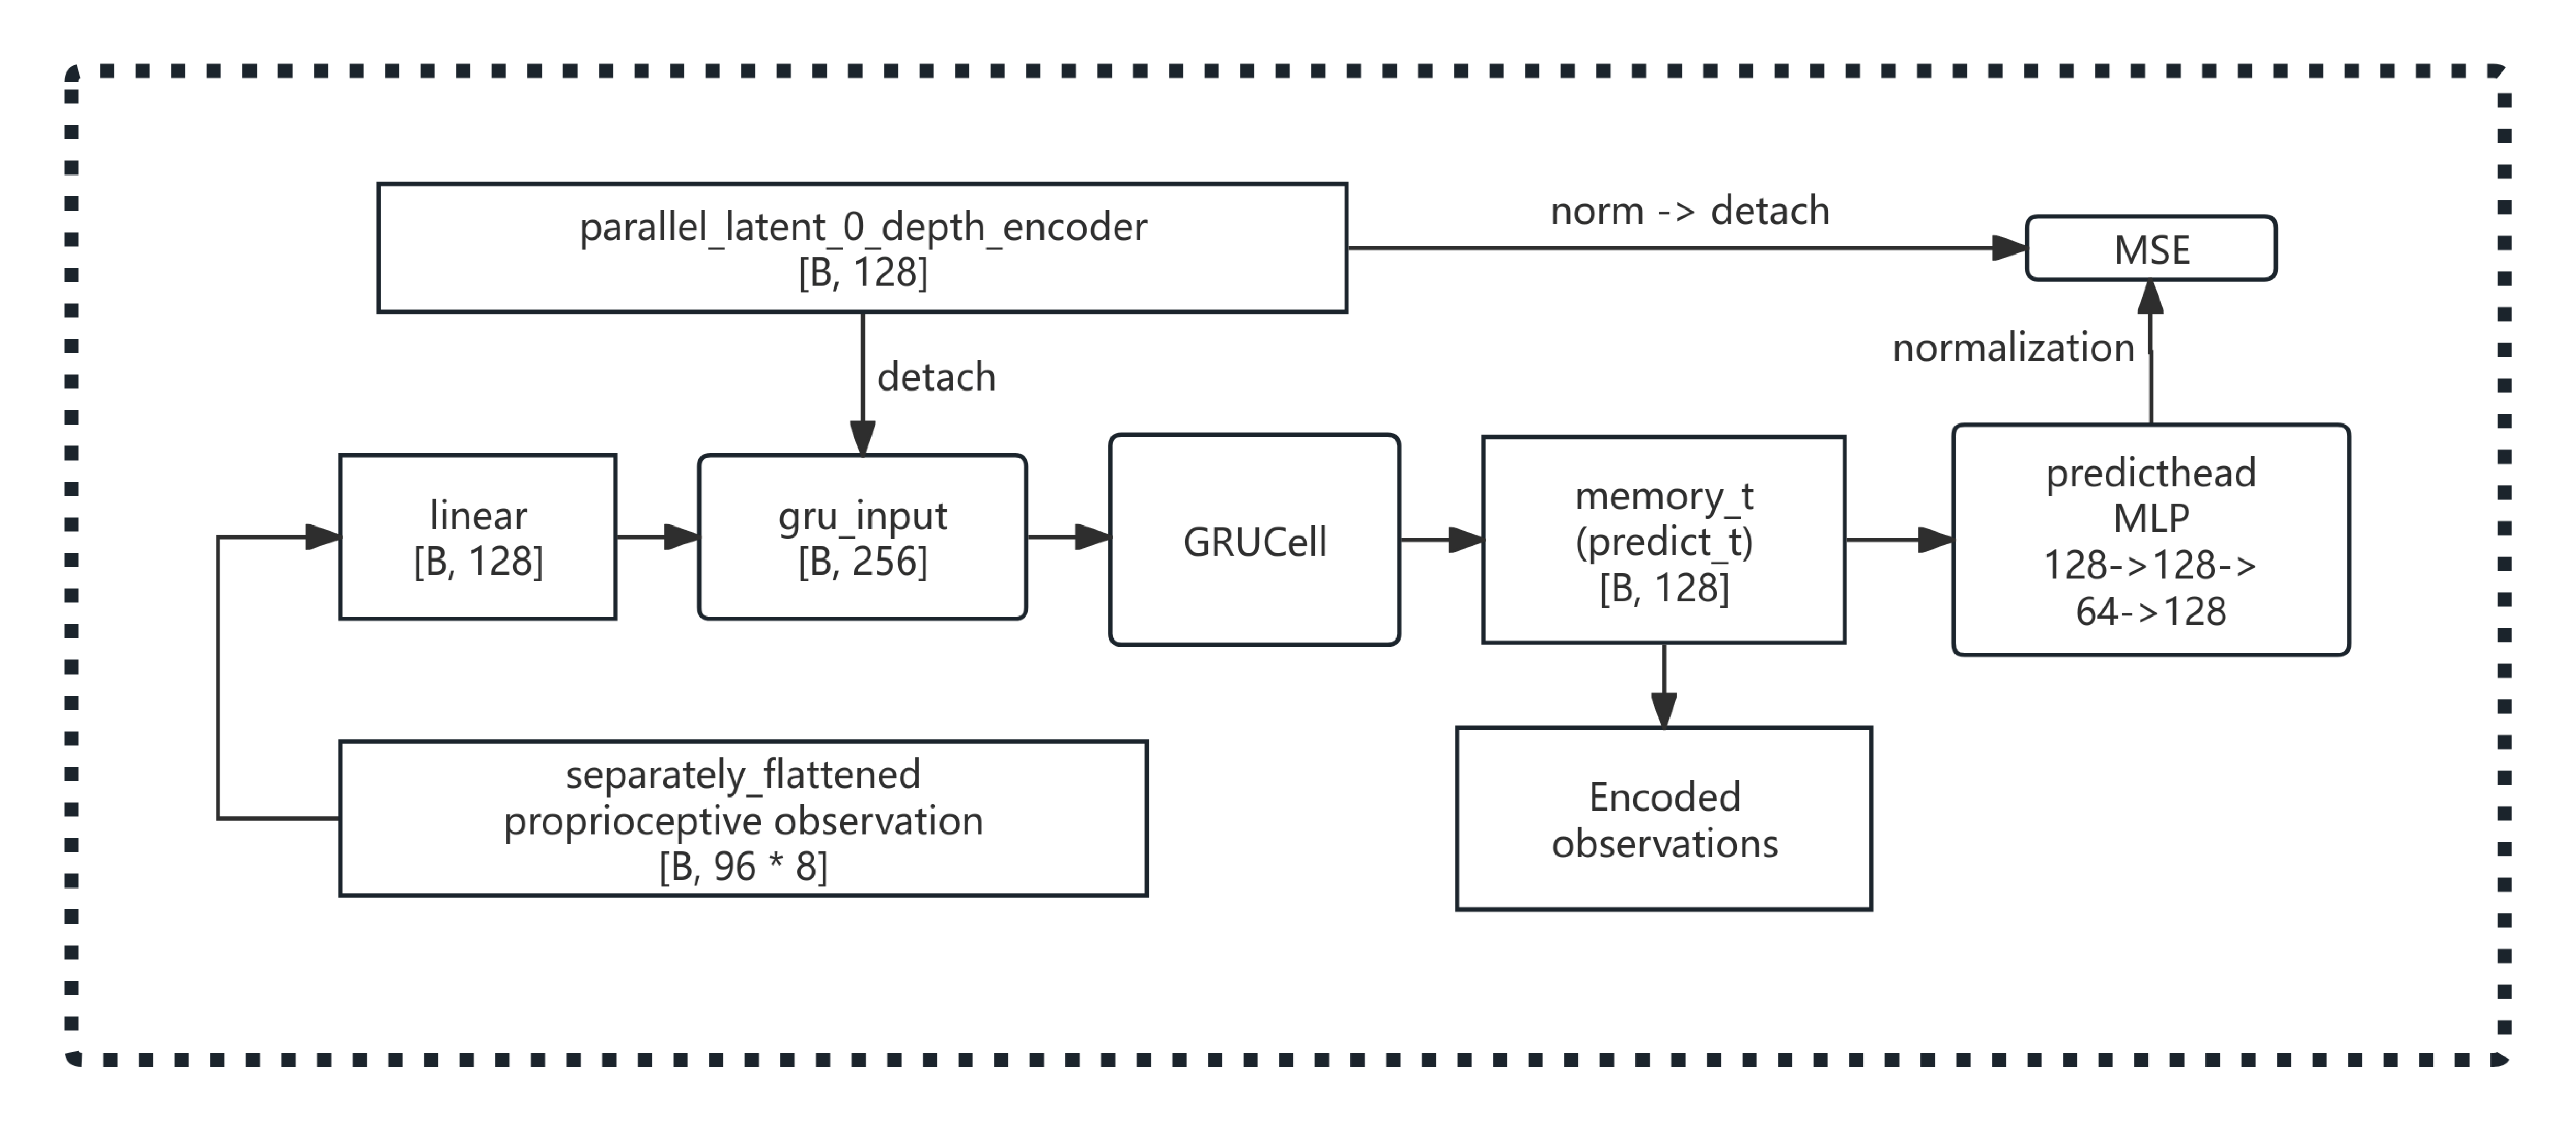
\includegraphics[width=0.85\textwidth]{figures/ch3_memory_module.pdf}
    \caption{Architecture of the memory module. The proprioceptive observations are projected to 128 dimensions and concatenated with the detached depth latent (128 dimensions) to form a 256-dimensional input to the GRU cell. The GRU hidden state (128 dimensions) is maintained across time steps and serves as the memory latent output. The consistency head produces a prediction target from the memory state, which is compared against the depth latent via the consistency loss.}
    \label{fig:memory_module}
\end{figure}

\subsection{Memory Consistency Loss}
\label{sec:consistency_loss}

A key challenge in training recurrent memory modules for locomotion is ensuring that the hidden state encodes meaningful information. Without explicit supervision, the GRU hidden state may degenerate into a representation that is useful for the policy's action selection but does not encode interpretable terrain features. This can lead to fragile memory representations that fail to generalize to new terrain configurations.

The proposed framework addresses this challenge through a \emph{memory consistency loss} that supervises the memory representation to predict the current depth latent. The consistency head is a multi-layer perceptron (MLP) that maps the memory hidden state to the depth latent space:
\begin{equation}
    \hat{\mathbf{z}}_t^d = f_{\text{head}}(\mathbf{m}_t) = W_3 \, \text{ELU}(W_2 \, \text{ELU}(W_1 \mathbf{m}_t + \mathbf{b}_1) + \mathbf{b}_2) + \mathbf{b}_3
\end{equation}
where the hidden dimensions are $128 \rightarrow 128 \rightarrow 64 \rightarrow 128$, matching the depth latent dimension. The consistency loss is then:
\begin{equation}
    \mathcal{L}_{\text{cons}} = \text{MSE}\left(\frac{\hat{\mathbf{z}}_t^d}{\|\hat{\mathbf{z}}_t^d\|}, \, \frac{\text{sg}(\mathbf{z}_t^d)}{\|\text{sg}(\mathbf{z}_t^d)\|}\right)
    \label{eq:consistency_loss}
\end{equation}
where both the prediction and the target are L2-normalized before computing the MSE. The normalization ensures that the loss measures the directional agreement between the memory prediction and the depth latent, rather than their magnitudes. The stop-gradient on $\mathbf{z}_t^d$ prevents the consistency loss from affecting the depth encoder's training.

\paragraph{Design Rationale.}
The consistency loss was arrived at after an unsuccessful attempt to train the memory module with a \emph{future prediction} objective---predicting the depth latent 1 second into the future. This approach failed for three reasons: (1)~the learning signal was insufficient, as predicting a precise future state from a noisy current observation is inherently difficult; (2)~the robot's body pose changes dramatically over 1 second in parkour, making the target depth latent highly variable; and (3)~predicting a single future time point provides a sparse and discontinuous training signal.

The current design---predicting the \emph{current} depth latent from the memory state---addresses these issues. The current depth latent is a stable, well-defined target that provides a dense learning signal at every time step. The key insight is that by requiring the memory to predict the current depth representation, the consistency loss forces the memory to encode a terrain interpretation that is consistent with the current visual observation. This terrain interpretation persists in the GRU hidden state even after the visual observation has changed, providing the policy with a stable terrain representation that is grounded in but not limited to the current depth input.

The consistency loss is incorporated into the PPO training objective as an auxiliary loss:
\begin{equation}
    \mathcal{L}_{\text{total}} = \mathcal{L}_{\text{PPO}} + \lambda_{\text{cons}} \cdot \mathcal{L}_{\text{cons}}
\end{equation}
where $\lambda_{\text{cons}}$ is a weighting coefficient. The consistency loss is computed for both the actor and critic encoders (which share the same architecture but maintain separate hidden states), and the total consistency loss is the average of the two.

\subsection{Qualitative Behavioral Effects}
\label{sec:memory_effects}

The memory module produces two notable behavioral effects that demonstrate its role in terrain understanding:

\paragraph{Conservative initial behavior.}
At the beginning of each episode, the GRU hidden state is initialized to zero, meaning the memory has no terrain information. However, the velocity commands immediately require the robot to move forward. The policy resolves this conflict by adopting a conservative locomotion strategy in the first few steps: it lifts its feet significantly higher than normal, effectively ``stepping blind'' with elevated foot clearance. This behavior is not a training artifact but rather a rational strategy: when the memory is empty, the policy has no information about the terrain ahead and compensates by increasing the safety margin for foot placement. As the GRU accumulates terrain information over the first few steps, the foot clearance gradually decreases to a normal level.

\paragraph{Confident terrain-adapted locomotion.}
After the memory has accumulated sufficient terrain information (typically within 3--5 steps), the policy transitions to terrain-adapted locomotion: it walks smoothly and efficiently on flat terrain, steps precisely on stairs, and adjusts its gait proactively when approaching obstacles. This transition from conservative to confident behavior indicates that the memory module is effectively encoding and maintaining terrain information, and that the policy has learned to modulate its behavior based on the information content of the memory state.

These behavioral patterns provide qualitative evidence that the memory consistency loss successfully forces the GRU hidden state to encode meaningful terrain representations. Without the consistency loss, the GRU hidden state would be free to encode arbitrary information that is useful for action selection but not necessarily terrain-related, potentially leading to a memory representation that is brittle and fails to generalize.

%% ============================================================
\section{Attention Module}
\label{sec:attention_module}
%% ============================================================

\subsection{Motivation}

While the depth image provides comprehensive spatial information about the terrain, not all regions of the depth image are equally important for the current locomotion decision. When the robot is approaching a gap, the region immediately ahead of its feet is far more critical than the distant terrain; when navigating near a wall, the wall's position and orientation determine whether the robot should stop or turn; and when stepping onto a narrow foothold, the precise geometry of the foothold region requires more attention than the surrounding terrain.

Existing depth-based locomotion methods process the entire depth image uniformly through a convolutional encoder~\cite{zhu2024hiking,zhuang2024humanoidparkour}, treating all spatial regions with equal importance. This uniform processing has two limitations: (1)~computational resources are wasted on irrelevant terrain regions, and (2)~the encoder may fail to capture fine-grained features in critical regions because its capacity is spread across the entire image. He et al.~\cite{he2024attentionmap} demonstrated that attention-based terrain encoding can improve locomotion generalization by selectively focusing on the most relevant terrain features, but their approach processes a single heightmap observation and does not address the multi-frame, multi-modal setting of the proposed framework.

The proposed attention module addresses these limitations through a cross-attention mechanism that uses the robot's current proprioceptive state as a query to selectively attend to the most task-relevant regions of the depth image. This design enables the policy to dynamically adjust its spatial focus based on the current locomotion context---for example, attending to nearby obstacles when approaching a gap, or focusing on wall structures when navigating confined spaces.

\subsection{Network Architecture}

The attention module implements a cross-attention mechanism between the proprioceptive observations (query) and the depth image spatial features (key and value). The architecture is as follows:

\begin{enumerate}
    \item \textbf{Key/Value construction.} The depth observation tensor $\mathbf{D}_t \in \mathbb{R}^{F \times H_d \times W_d}$ (where $F=8$, $H_d=36$, $W_d=64$) is reshaped into a sequence of spatial feature vectors. Each spatial position $(h, w)$ in the depth image has an $F$-dimensional feature vector (one value per temporal frame), and the entire image produces $L = H_d \times W_d = 2304$ such vectors:
    \begin{equation}
        \mathbf{K}_t = \mathbf{V}_t = \text{reshape}(\text{permute}(\mathbf{D}_t)) \in \mathbb{R}^{L \times d_a}
    \end{equation}
    where $d_a = F = 8$ is the attention embedding dimension. The constraint that the attention embedding dimension equals the number of depth frames ensures that the depth features can be directly used as key/value vectors without an additional projection layer, reducing the parameter count.

    \item \textbf{Query construction.} The proprioceptive observations are projected to the attention embedding dimension:
    \begin{equation}
        \mathbf{q}_t = W_q \mathbf{o}_t^{\text{prop}} + \mathbf{b}_q, \quad \mathbf{q}_t \in \mathbb{R}^{d_a}
    \end{equation}
    The query is then unsqueezed to add a sequence dimension: $\mathbf{Q}_t = \mathbf{q}_t^{\top} \in \mathbb{R}^{1 \times d_a}$.

    \item \textbf{Multi-head cross-attention.} The query, key, and value are processed by a multi-head attention layer with $N_h = 2$ heads:
    \begin{equation}
        \text{Attn}(\mathbf{Q}_t, \mathbf{K}_t, \mathbf{V}_t) = \text{softmax}\left(\frac{\mathbf{Q}_t \mathbf{K}_t^\top}{\sqrt{d_a / N_h}}\right) \mathbf{V}_t
    \end{equation}
    The output is a single vector $\mathbf{a}_t \in \mathbb{R}^{d_a}$ obtained by squeezing the sequence dimension. The two attention heads enable the module to learn two distinct spatial attention patterns---for example, one head may specialize in attending to nearby terrain features (relevant for immediate foot placement), while the other may attend to distant terrain features (relevant for trajectory planning).
\end{enumerate}

\begin{figure}[t]
    \centering
    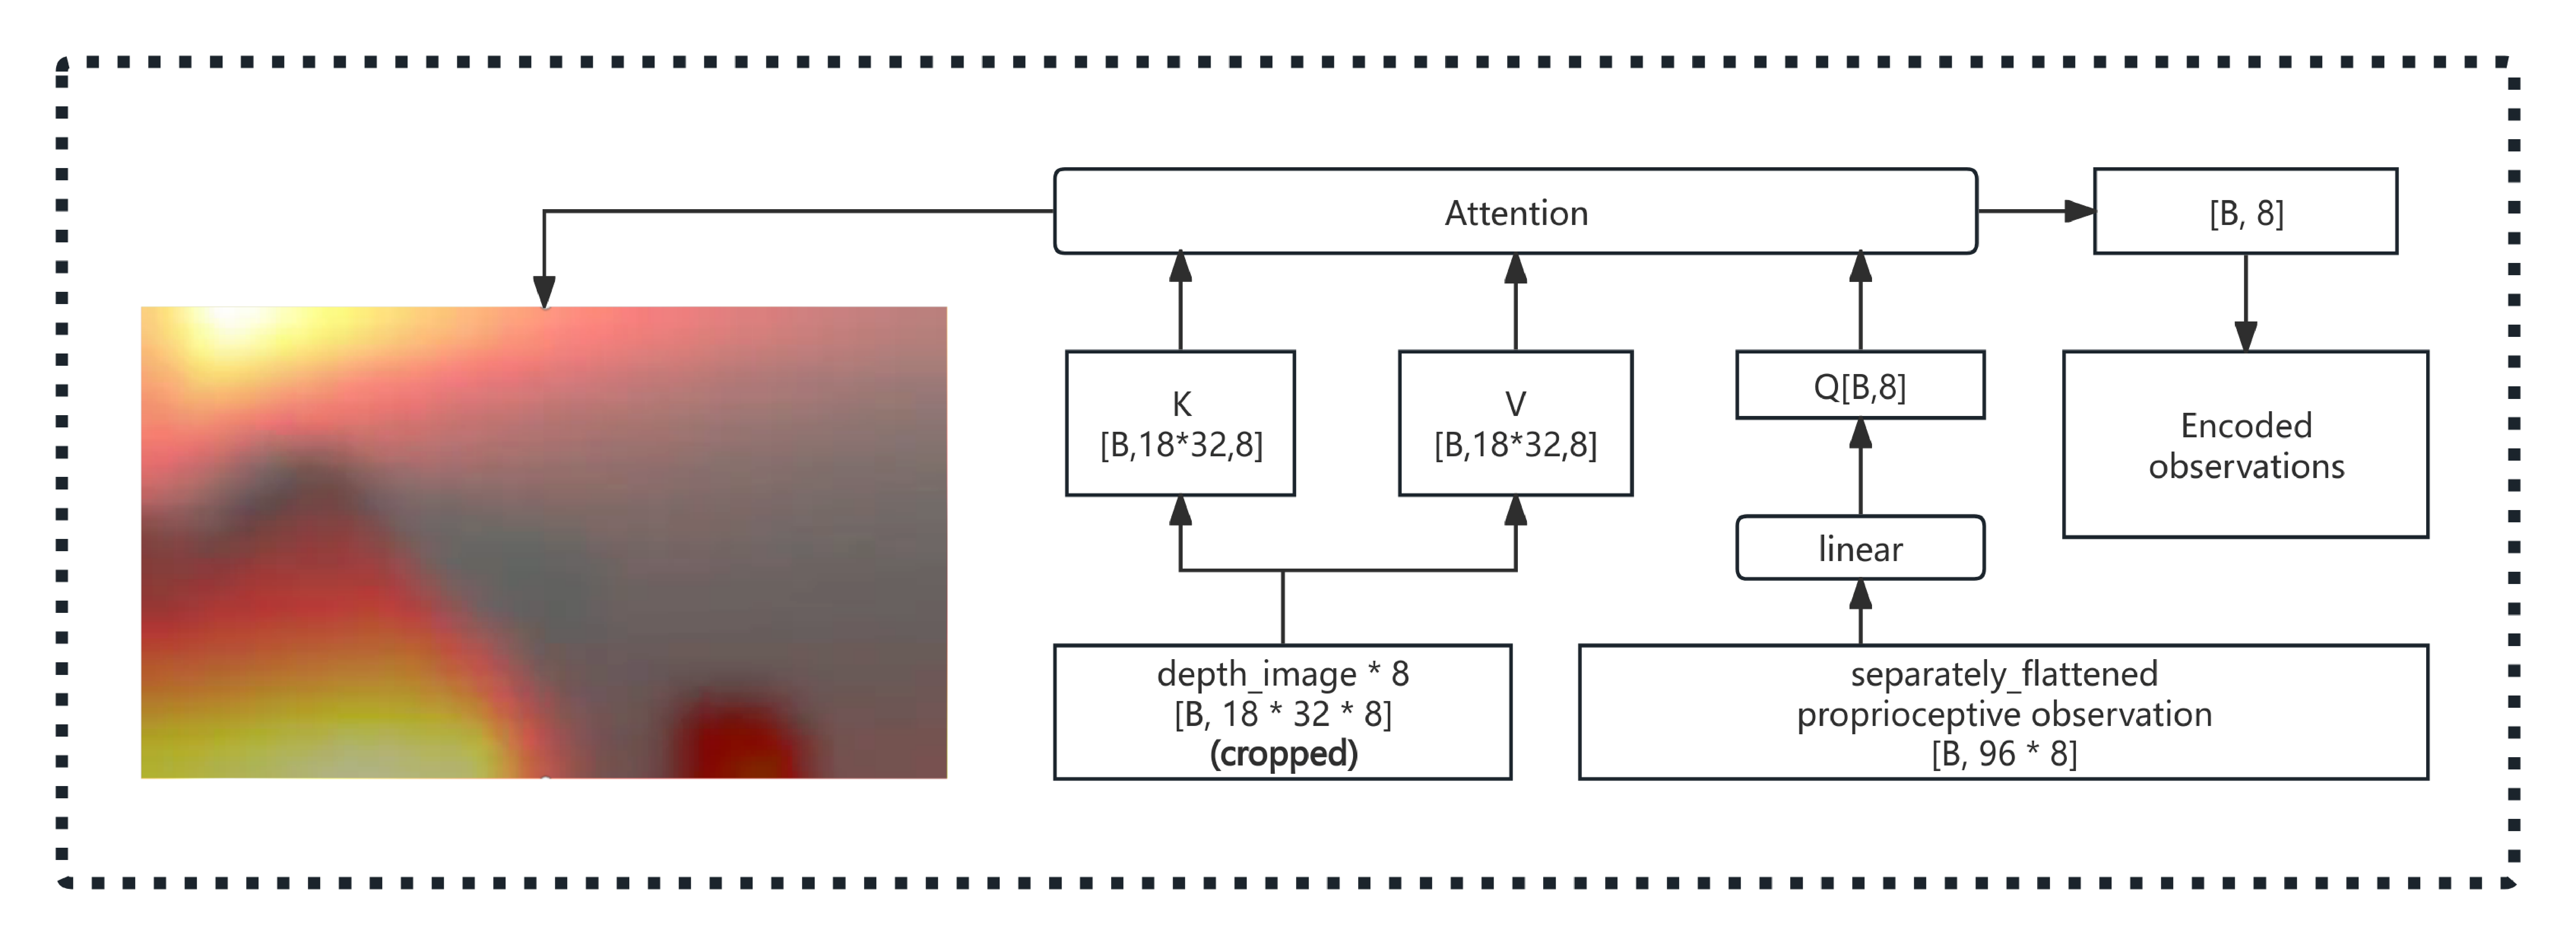
\includegraphics[width=0.85\textwidth]{figures/ch3_attention_module.pdf}
    \caption{Architecture of the cross-attention module. The depth image is reshaped into a sequence of $L = H_d \times W_d$ spatial feature vectors, each of dimension $d_a = F$ (the number of depth frames). The proprioceptive observations are projected to the same dimension and used as a query. Multi-head cross-attention (2 heads) produces an attention output $\mathbf{a}_t \in \mathbb{R}^{d_a}$. The attention weights can be reshaped back to the spatial dimensions of the depth image for visualization.}
    \label{fig:attention_module}
\end{figure}

The attention weights can be reshaped from $(N_h, 1, L)$ to $(N_h, H_d, W_d)$ to produce spatial attention maps over the depth image. These attention maps provide interpretable insights into which terrain regions the policy attends to when making locomotion decisions, enabling qualitative analysis of the policy's spatial focus.

\subsection{Qualitative Behavioral Effects}
\label{sec:attention_effects}

Visualization of the attention weights reveals that the policy learns meaningful spatial attention patterns that adapt to different terrain scenarios:

\paragraph{Obstacle avoidance.}
When the depth image contains obstacles that could affect the robot's posture or cause tripping, the attention weights concentrate on these obstacle regions. The policy learns to attend to the spatial extent and proximity of obstacles, enabling it to adjust its foot placement and body posture proactively rather than reactively. This is particularly important for small obstacles (e.g., stones, low steps) that occupy a small portion of the depth image but have a disproportionate impact on locomotion stability.

\paragraph{Wall avoidance.}
When the depth image shows a wall ahead, the attention weights focus on the wall region, and the policy learns to stop forward motion rather than colliding with the wall. This behavior demonstrates that the attention module enables the policy to recognize and respond to terrain features that require a qualitative change in locomotion strategy (from forward motion to stopping), rather than merely adjusting the parameters of a fixed locomotion pattern.

\paragraph{Two-stage gap crossing.}
For gap-crossing scenarios, the attention weights reveal a two-stage decision process. In the first stage, when the gap is still at a distance, the attention focuses on the gap's far edge, and the policy walks toward the gap edge (rather than attempting to leap from a distance). In the second stage, when the robot is at the gap edge, the attention shifts to the gap's geometry (width, depth), and the policy adjusts its center of mass and executes a large step to cross the gap. This two-stage behavior---approach then cross---is more robust than attempting to cross the gap from an arbitrary distance, as it ensures that the robot has optimal footing and balance before committing to the crossing maneuver.

\paragraph{Comparison with attention-free AMP-only policies.}
Policies trained with AMP but without the attention module exhibit a characteristic limitation: they learn natural locomotion postures through the AMP discriminator and basic obstacle avoidance through the depth encoder, but they fail to attend to small, localized terrain features such as stones or low steps near the robot's feet. This is a well-known limitation of current AMP-based locomotion methods---the AMP reward encourages natural motion style but does not provide the spatial selectivity needed to focus on critical terrain regions. The attention module addresses this limitation by enabling the policy to selectively amplify the representation of important terrain features, ensuring that even small obstacles receive sufficient processing capacity.

%% ============================================================
\section{Mixture-of-Experts Module}
\label{sec:moe_module}
%% ============================================================

\subsection{Motivation}

Parkour requires the robot to execute a diverse repertoire of locomotion skills---walking on flat terrain, climbing stairs, leaping across gaps, navigating slopes, and avoiding walls---often in rapid succession as the terrain changes. A single monolithic policy network may struggle to simultaneously master all these skills, as the optimal locomotion strategy for one terrain type may conflict with the optimal strategy for another (e.g., the high-step strategy for stairs vs.\ the low-swing strategy for flat walking).

Existing approaches to multi-skill parkour employ explicit skill decomposition: Extreme Parkour~\cite{cheng2024extremeparkour} and Robot Parkour Learning~\cite{zhuang2024robotparkour} train separate skill policies for each maneuver type and use a high-level planner to select and parameterize skills. While effective, this skill-chaining paradigm requires manual skill definition, careful skill boundary design, and a separate high-level policy, increasing the engineering complexity and limiting the system's ability to learn novel skill combinations.

The proposed framework employs a Mixture-of-Experts (MoE) architecture as an alternative to explicit skill decomposition. In the MoE paradigm, the policy network contains multiple expert sub-networks, each of which can specialize in a different locomotion strategy, and a gating network that dynamically selects which experts to activate for each input. This design enables the policy to learn diverse locomotion skills end-to-end without requiring explicit skill labels or a high-level skill selector.

\subsection{Network Architecture}

The MoE module replaces the standard MLP actor and critic heads with MoE layers. Each MoE layer consists of two components:

\begin{enumerate}
    \item \textbf{Gating network.} A linear layer maps the input to a distribution over experts:
    \begin{equation}
        \mathbf{g}_t = \text{softmax}(W_g \mathbf{x}_t + \mathbf{b}_g), \quad \mathbf{g}_t \in \mathbb{R}^{N_e}
    \end{equation}
    where $N_e = 8$ is the number of experts. The gate scores $\mathbf{g}_t$ represent the relative importance of each expert for the current input.

    \item \textbf{Expert networks.} Each expert $e$ is an MLP with hidden dimensions $[256, 256, 256]$ and an output dimension matching the action space (for the actor) or value space (for the critic). All experts share the same architecture but have independent parameters.

    \item \textbf{Weighted mixing.} The expert outputs are combined according to the gate scores:
    \begin{equation}
        \mathbf{y}_t = \sum_{e=1}^{N_e} g_{t,e} \cdot \mathbf{y}_{t,e} = \sum_{e=1}^{N_e} g_{t,e} \cdot f_e(\mathbf{x}_t)
    \end{equation}
    where $f_e$ is the $e$-th expert network and $g_{t,e}$ is the gate score for expert $e$ at time $t$. This soft mixing allows multiple experts to contribute to the output, enabling smooth interpolation between specialized strategies.
\end{enumerate}

\begin{figure}[t]
    \centering
    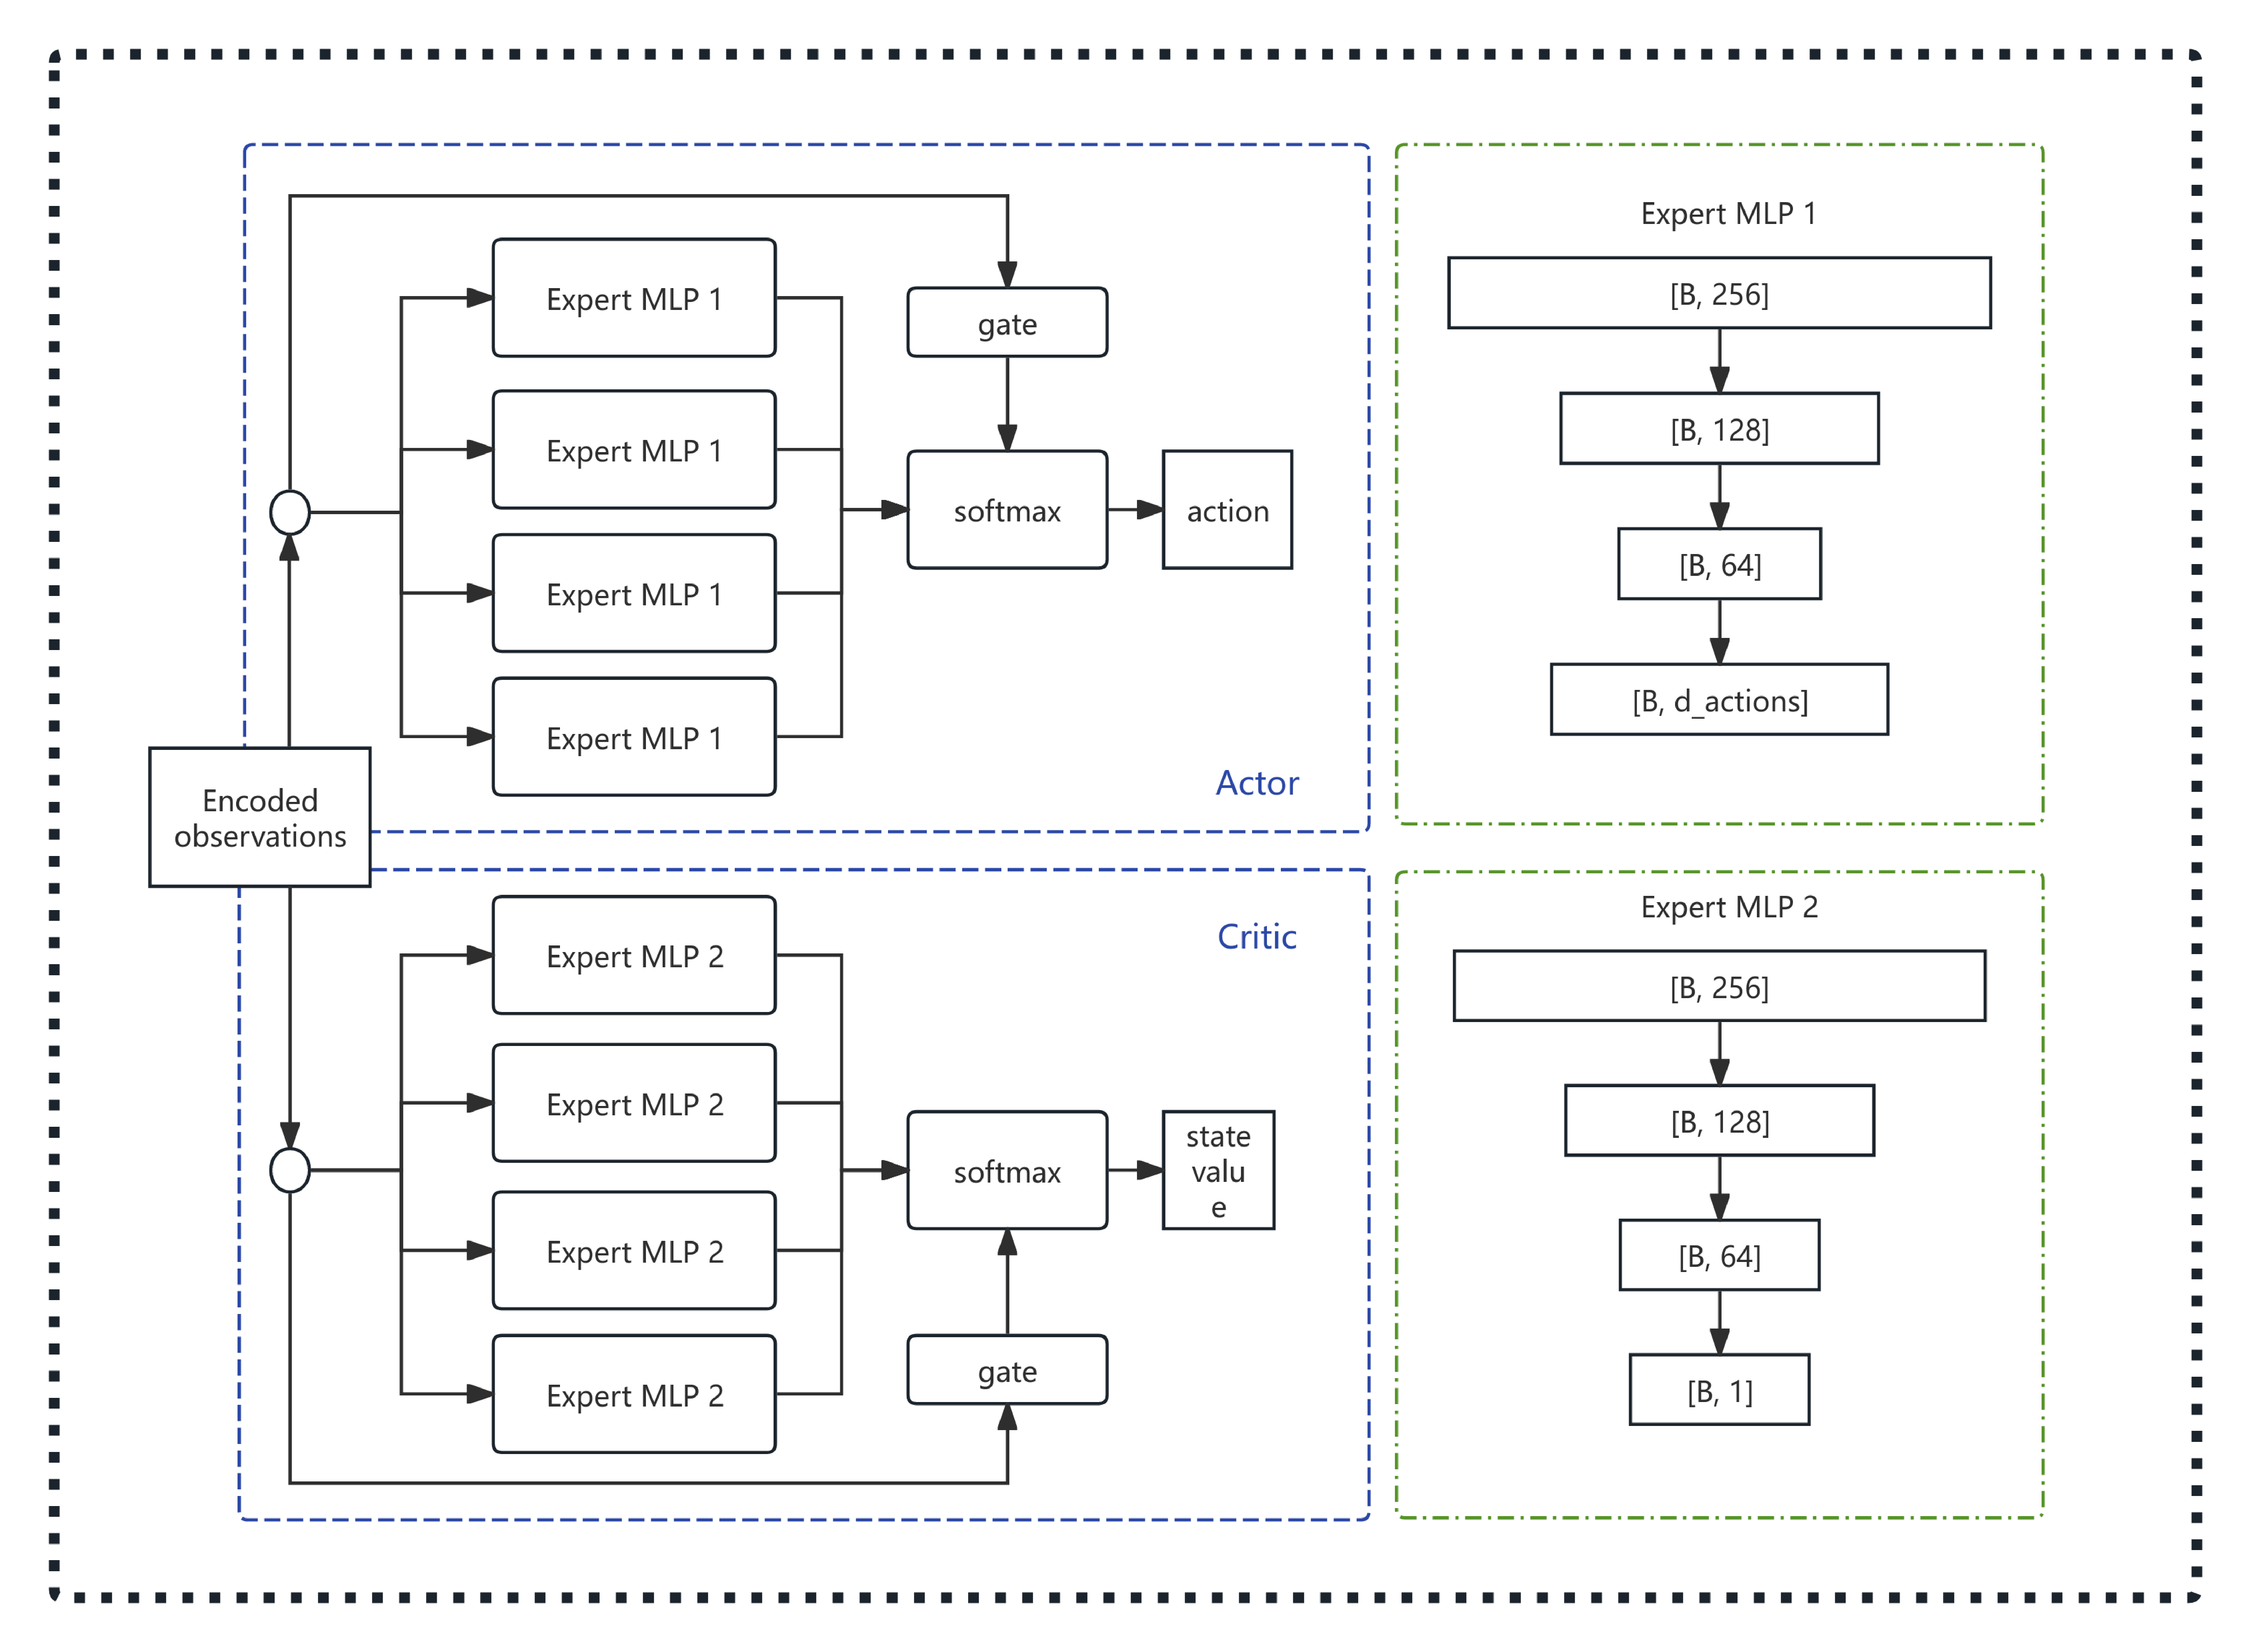
\includegraphics[width=0.75\textwidth]{figures/ch3_moe_module.pdf}
    \caption{Architecture of the Mixture-of-Experts layer. The input $\mathbf{x}_t$ is processed by a gating network that produces a softmax distribution over $N_e = 8$ experts. Each expert is an MLP with hidden dimensions $[256, 256, 256]$. The expert outputs are combined by weighted summation according to the gate scores. Both the actor and critic heads use independent MoE layers.}
    \label{fig:moe_module}
\end{figure}

The actor and critic each use an independent MoE layer with separate gating networks and expert parameters. This allows the actor and critic to develop different expert specializations: the actor's experts may specialize in different locomotion strategies (e.g., one expert for high-step climbing, another for flat walking), while the critic's experts may specialize in evaluating different terrain types.

\subsection{Comparison with Skill-Chaining Approaches}

The MoE architecture offers several advantages over the skill-chaining paradigm used in Extreme Parkour~\cite{cheng2024extremeparkour} and Robot Parkour Learning~\cite{zhuang2024robotparkour}:

\begin{enumerate}
    \item \textbf{No manual skill definition.} The MoE module does not require pre-defined skill categories or skill-specific reward functions. The expert specializations emerge automatically during training, driven by the diversity of the training terrain and the overall reward structure.

    \item \textbf{Smooth skill transitions.} The soft mixing of expert outputs enables smooth transitions between locomotion strategies, avoiding the discontinuities that can arise when switching between discrete skill policies.

    \item \textbf{End-to-end training.} The entire policy---including the encoder, MoE heads, and gating network---is trained jointly with a single PPO objective, simplifying the training pipeline compared to the multi-stage training required for skill-chaining approaches.

    \item \textbf{Scalability.} Adding more experts increases the model's capacity without changing the inference cost per expert, as each expert is evaluated independently. The gate computation adds negligible overhead.
\end{enumerate}

The primary limitation of the MoE approach is that the expert specializations are not guaranteed to be interpretable or well-separated: multiple experts may learn similar strategies, or a single expert may dominate the gate scores. However, the soft mixing mechanism mitigates this concern by ensuring that the output is always a reasonable combination of expert opinions, even if the expert specializations are not perfectly distinct.

%% ============================================================
\section{Adversarial Motion Prior Module}
\label{sec:amp_module}
%% ============================================================

\subsection{Motivation}

Reinforcement learning policies trained with pure task rewards often produce locomotion behaviors that are functionally correct but visually unnatural---the robot may shuffle its feet, exhibit jerky joint motions, or adopt awkward body postures that achieve the task objective but are energetically inefficient and potentially damaging to the hardware. In parkour scenarios, this problem is particularly acute because the diverse terrain types encourage the policy to adopt a wide range of locomotion strategies, some of which may be functional but physically implausible.

Adversarial Motion Priors (AMP)~\cite{peng2021amp} provide a principled solution to this problem by training a discriminator network that distinguishes between the policy's motion (``fake'') and reference motion data (``real''). The policy receives an adversarial reward that encourages it to produce motions that are indistinguishable from the reference data, effectively learning a style prior that regularizes the task-driven policy toward natural, human-like motion.

\subsection{AMP Framework}

The AMP module consists of a discriminator network $D_\phi$ that is trained concurrently with the policy. The discriminator receives a window of motion features and outputs a probability that the motion is ``real'' (from the reference dataset) rather than ``fake'' (from the policy). The AMP reward for the policy is:
\begin{equation}
    r_t^{\text{AMP}} = -\log(1 - D_\phi(\mathbf{s}_t^{\text{amp}})) + \log(D_\phi(\mathbf{s}_t^{\text{ref}}))
\end{equation}
where $\mathbf{s}_t^{\text{amp}}$ denotes the motion features from the policy and $\mathbf{s}_t^{\text{ref}}$ denotes the motion features from the reference dataset. The discriminator is trained to maximize its classification accuracy, while the policy is trained to maximize the AMP reward (i.e., to fool the discriminator).

\subsection{Observation Groups for AMP}

The AMP discriminator processes two observation groups with identical structure but different data sources:

\begin{table}[t]
\centering
\caption{AMP observation components for both the policy (amp\_policy) and reference (amp\_reference) groups. Each component is repeated over a history window of $H_{\text{amp}}=10$ time steps.}
\label{tab:amp_obs}
\begin{tabular}{llc}
\toprule
\textbf{Component} & \textbf{Description} & \textbf{Dim. per step} \\
\midrule
Projected gravity & Gravity vector in body frame & 3 \\
Joint positions (relative) & Current joint pos.\ minus default pos. & 29 \\
Joint velocities (relative) & Joint velocities (scaled by 0.05) & 29 \\
Base linear velocity & Linear velocity in body frame & 3 \\
Base angular velocity & Angular velocity in body frame & 3 \\
\midrule
\textbf{Total per step} & & \textbf{67} \\
\textbf{Total with history} & $67 \times H_{\text{amp}}$ & \textbf{670} \\
\bottomrule
\end{tabular}
\end{table}

The \texttt{amp\_policy} observation group samples motion features from the policy's current trajectory, while the \texttt{amp\_reference} observation group samples motion features from the retargeted reference dataset. The reference dataset consists of self-collected motion capture data of walking, running, and stair-climbing motions, retargeted to the robot's morphology using a general motion retargeting method~\cite{araujo2024retargeting}. The data collection and retargeting process is described in detail in Chapter~4.

\subsection{Integration with PPO Training}

The AMP reward is combined with the task reward to form the total reward signal for PPO training:
\begin{equation}
    r_t = r_t^{\text{task}} + w_{\text{AMP}} \cdot r_t^{\text{AMP}}
\end{equation}
where $w_{\text{AMP}}$ is a weighting coefficient that balances the task objective and the motion style objective. The discriminator is updated concurrently with the policy using a separate Adam optimizer, following the standard AMP training procedure~\cite{peng2021amp}.

The AMP discriminator is trained with a gradient penalty to prevent it from becoming overly confident, which could lead to vanishing gradients for the policy. The discriminator loss is:
\begin{equation}
    \mathcal{L}_D = -\mathbb{E}[\log D_\phi(\mathbf{s}^{\text{ref}})] - \mathbb{E}[\log(1 - D_\phi(\mathbf{s}^{\text{amp}}))] + \lambda_{\text{gp}} \cdot \mathcal{L}_{\text{gp}}
\end{equation}
where $\mathcal{L}_{\text{gp}}$ is the gradient penalty term and $\lambda_{\text{gp}}$ is its weighting coefficient.

\subsection{Comparison with Existing AMP Applications}

Most existing AMP-based locomotion methods~\cite{peng2021amp,zhang2024advdiscriminators} use publicly available motion capture datasets (e.g., AMASS) that primarily contain walking and running on flat ground. While these datasets provide a good style prior for flat-terrain locomotion, they lack the diversity of motion patterns needed for parkour---stair climbing, high-stepping, cautious approach walking, and dynamic leaping are not well-represented in standard motion capture datasets.

The proposed framework addresses this limitation by using self-collected motion capture data that specifically targets parkour-relevant motions. The reference dataset includes walking, running, and stair-climbing motions captured from human actors using a motion capture system, and retargeted to the robot's morphology using a general motion retargeting method~\cite{araujo2024retargeting}. This ensures that the AMP discriminator provides a style prior that is both natural (grounded in real human motion) and relevant (covering the motion patterns needed for parkour). The retargeting process accounts for differences in body proportions and joint limits between the human actor and the robot, producing reference motions that are feasible for the robot's embodiment.

Furthermore, the proposed framework applies symmetric augmentation to the reference dataset: each reference motion is mirrored left-to-right using a joint mapping that swaps corresponding left and right joints. This doubles the effective size of the reference dataset and encourages the AMP discriminator to learn symmetric motion patterns, which is important for bipedal locomotion where left and right steps should be stylistically similar.

%% ============================================================
\section{Implementation Details}
\label{sec:implementation}
%% ============================================================

This section describes the implementation details of the proposed framework, including the reward function design, environment configuration, sensor randomization, domain randomization, and training procedure. These details are critical for reproducibility and for understanding the design choices that differentiate the proposed method from ablation variants.

\subsection{Reward Function Design}
\label{sec:reward_function}

The reward function is composed of three categories: task rewards that encourage goal-directed behavior, regularization rewards that promote smooth and efficient motion, and safety rewards that prevent dangerous states. The complete reward function is listed in Table~\ref{tab:reward_terms}.

\begin{table}[t]
\centering
\caption{Complete reward function components. Positive weights indicate rewards, negative weights indicate penalties.}
\label{tab:reward_terms}
\footnotesize
\begin{tabular}{@{}lp{3.2cm}rp{7cm}@{}}
\toprule
\textbf{Category} & \textbf{Term} & \textbf{Weight} & \textbf{Description} \\
\midrule
\multirow{6}{*}{Task} & track\_lin\_vel\_xy & $+2.0$ & Track commanded linear velocity (exp.\ kernel, $\sigma=0.5$) \\
 & track\_ang\_vel\_z & $+2.0$ & Track commanded angular velocity (exp.\ kernel, $\sigma=0.5$) \\
 & heading\_error & $-1.0$ & Penalize heading deviation from command \\
 & dont\_wait & $-0.5$ & Penalize standing still when forward command is active \\
 & is\_alive & $+3.0$ & Reward for surviving each step \\
 & stand\_still & $-0.3$ & Penalize moving when no command (offset=4.0) \\
\midrule
\multirow{12}{*}{Regularization} & volume\_points\_penetration & $-4.0$ & Penalize foot volume penetrating virtual obstacles \\
 & feet\_air\_time & $+0.5$ & Reward swing foot air time (bipedal stepping) \\
 & feet\_slide & $-0.4$ & Penalize foot sliding on contact (threshold=1.0) \\
 & joint\_deviation\_hip & $-0.5$ & Penalize hip yaw/roll deviation from default \\
 & ang\_vel\_xy\_l2 & $-0.05$ & Penalize base roll/pitch angular velocity \\
 & dof\_torques\_l2 & $-1.5 \times 10^{-7}$ & Penalize joint torques (hip, knee, ankle) \\
 & dof\_acc\_l2 & $-1.25 \times 10^{-7}$ & Penalize joint accelerations \\
 & dof\_vel\_l2 & $-1.0 \times 10^{-4}$ & Penalize joint velocities \\
 & action\_rate\_l2 & $-0.005$ & Penalize action change between steps \\
 & flat\_orientation\_l2 & $-3.0$ & Penalize base orientation deviation from horizontal \\
 & pelvis\_orientation\_l2 & $-3.0$ & Penalize pelvis orientation deviation \\
 & feet\_flat\_ori & $-0.4$ & Penalize foot orientation misalignment on contact \\
\midrule
\multirow{7}{*}{Regularization (cont.)} & feet\_at\_plane & $-0.1$ & Penalize foot height error vs.\ terrain plane \\
 & feet\_close\_xy & $+0.4$ & Reward feet at appropriate lateral distance ($\sigma^2=0.05$) \\
 & energy & $-5.0 \times 10^{-5}$ & Penalize mechanical power (torque$\times$velocity) \\
 & freeze\_upper\_body & $-0.004$ & Penalize upper body joint deviation (L1 norm) \\
\midrule
\multirow{4}{*}{Safety} & dof\_pos\_limits & $-1.0$ & Penalize joint position limit violations \\
 & dof\_vel\_limits & $-1.0$ & Penalize joint velocity limit violations (soft ratio=0.9) \\
 & torque\_limits & $-0.01$ & Penalize torque exceeding 80\% of limit \\
 & undesired\_contacts & $-1.0$ & Penalize non-foot contact forces $>1.0$~N \\
\bottomrule
\end{tabular}
\end{table}

Several reward terms warrant additional discussion:

\paragraph{Volume points penetration.}
This term is a key safety mechanism for parkour. A set of 3D sample points is generated around each ankle in a grid pattern ($10 \times 5 \times 2$ points, spanning a volume of $0.15 \times 0.06 \times 0.04$~m around the foot). These points are checked against virtual obstacles generated from the terrain mesh (specifically, cylindrical approximations of terrain edges). The penalty is proportional to both the penetration depth and the velocity of the penetrating points, encouraging the robot to avoid obstacles and to move slowly when near them:
\begin{equation}
    r_{\text{pen}} = -w_{\text{pen}} \sum_{i} \mathbb{1}[d_i > \epsilon] \cdot (\|\mathbf{v}_i\| + \epsilon_v) \cdot d_i
\end{equation}
where $d_i$ is the penetration depth of point $i$, $\mathbf{v}_i$ is its velocity, and $w_{\text{pen}} = 4.0$. This reward term is particularly important for ensuring that the robot does not step through virtual obstacles such as terrain edges and low walls, which are represented as collision-free visual elements in the simulation.

\paragraph{Feet air time (bipedal).}
Unlike the standard feet air time reward used for quadrupedal locomotion, the bipedal version rewards the minimum air time of the swing foot during single-stance phases. This encourages the robot to take proper steps with adequate foot clearance, rather than shuffling or dragging its feet.

\paragraph{Feet close XY.}
This term encourages the robot to maintain an appropriate lateral distance between its feet using a Gaussian kernel:
\begin{equation}
    r_{\text{close}} = w_{\text{close}} \left(\exp\left(-\frac{\max(\tau - d_{\text{lat}}, 0)}{\sigma^2}\right) - 1\right)
\end{equation}
where $d_{\text{lat}}$ is the lateral foot distance, $\tau = 0.12$~m is the threshold, and $\sigma^2 = 0.05$. This prevents the robot from crossing its feet or walking with an excessively wide stance.

\paragraph{Freeze upper body.}
An L1-norm penalty on the deviation of upper body joints (shoulders, elbows, wrists, waist) from their default positions encourages the robot to keep its upper body still during locomotion. This is important for two reasons: (1)~it reduces the complexity of the whole-body coordination problem, allowing the policy to focus on lower-body locomotion; and (2)~it produces more natural-looking motion, as humans typically maintain a relatively stable upper body posture during walking and running.

\subsection{Environment Configuration}
\label{sec:env_config}

\subsubsection{Robot Configuration}

The robot is a Unitree G1 humanoid with 29 actuated degrees of freedom (excluding the floating base). The action space consists of target joint positions for all 29 joints, which are tracked by delayed PD actuators with configurable stiffness and damping. The robot is equipped with custom shoe attachments that modify the foot geometry and the contact dynamics, requiring adjusted reward parameters (e.g., the feet-at-plane height offset is increased from 0.035~m to 0.058~m to account for the shoe sole thickness).

\subsubsection{Terrain Configuration}

The training environment uses a terrain generator that produces 10 types of sub-terrains arranged in a $10 \times 20$ grid, with each sub-terrain measuring $8 \times 8$~m. The sub-terrain types and their proportions are listed in Table~\ref{tab:terrain_types}.

\begin{table}[t]
\centering
\caption{Terrain types used in training, with their proportions and key parameters.}
\label{tab:terrain_types}
\footnotesize
\begin{tabular}{@{}lp{1.5cm}p{4cm}p{4.5cm}@{}}
\toprule
\textbf{Type} & \textbf{Proportion} & \textbf{Key Parameters} & \textbf{Description} \\
\midrule
Perlin rough & 5\% & noise scale [0, 0.1] & Rough terrain with Perlin noise \\
Perlin rough (stand) & 5\% & noise scale [0, 0.1] & Rough terrain for standing practice \\
Square gaps & 10\% & gap 0.1--0.7~m, depth 0.4--0.6~m & Terrain with rectangular gaps \\
Pyramid stairs & 15\% & step height 0.05--0.23~m & Ascending stairs with Perlin noise \\
Pyramid stairs (high) & 10\% & step height 0.05--0.45~m & High ascending stairs \\
Inv.\ pyramid stairs & 15\% & step height 0.05--0.23~m & Descending stairs with Perlin noise \\
Inv.\ pyramid stairs (high) & 10\% & step height 0.05--0.45~m & High descending stairs \\
Discrete boxes & 10\% & height 0.05--0.45~m, width 0.8--1.5~m & Scattered box obstacles \\
Mesh boxes & 10\% & height 0.1--0.4~m & Dense small box obstacles \\
Inv.\ pyramid slope & 10\% & slope 0--0.7 & Sloped terrain with Perlin noise \\
\bottomrule
\end{tabular}
\end{table}

Each sub-terrain has a 30\% probability of generating virtual walls on each of its four edges, with a wall height of 5.0~m and thickness of 0.05~m. These walls create confined-space navigation scenarios that require the robot to stop or turn when encountering a wall. The terrain generator also produces virtual obstacles in the form of cylindrical approximations of terrain edges, which are used by the volume points penetration reward (Section~\ref{sec:reward_function}).

A terrain difficulty curriculum is applied during training: the terrain level (row index) assigned to each environment is determined by the robot's velocity tracking performance. Environments where the robot successfully tracks the commanded velocity are assigned to higher terrain levels (more difficult terrain), while environments where the robot fails are assigned to lower levels (easier terrain). This curriculum ensures that the policy is gradually exposed to increasingly challenging terrain configurations.

\subsubsection{Simulation Parameters}

The simulation uses a physics time step of $\Delta t_{\text{sim}} = 0.005$~s with a decimation factor of 4, resulting in a control period of $\Delta t = 0.02$~s (50~Hz control frequency). The episode length is 20 seconds (1000 control steps). The training uses 4096 parallel simulated environments, enabling efficient sample collection for PPO training.

\subsection{Sensor Randomization}
\label{sec:sensor_randomization}

Sensor randomization is a critical component for sim-to-real transfer, as it bridges the gap between the idealized sensor models in simulation and the noisy, delayed, and miscalibrated sensors on real hardware. The proposed framework applies extensive sensor randomization during training:

\paragraph{Camera offset randomization.}
The camera's extrinsic calibration (position and orientation relative to the torso link) is randomized at the start of each episode. The position offsets are sampled uniformly within specified ranges for each axis, and the orientation offsets are sampled similarly for roll, pitch, and yaw. This simulates the installation errors and mechanical vibrations that affect the camera's calibration on the real robot, forcing the policy to be robust to camera misalignment.

\paragraph{Depth noise pipeline.}
As described in Section~\ref{sec:depth_obs}, the depth images are processed through a multi-stage noise pipeline that includes crop-and-resize, Gaussian blur, depth normalization, additive Gaussian noise, and depth artifact noise. Each stage introduces a different type of sensor degradation, and the combination produces depth images that approximate the quality of real depth sensor output.

\paragraph{Frame delay randomization.}
A random delay of 0--1 frames is applied to the depth observation, simulating the processing and transmission latency of real depth sensors. This forces the policy to be robust to slightly outdated depth information, which is important for real-time deployment where sensor latency can vary.

\subsection{Domain Randomization}
\label{sec:domain_randomization}

In addition to sensor randomization, the proposed framework applies domain randomization to the physical properties of the simulation:

\paragraph{Physics material randomization.}
The friction and restitution coefficients of the robot's bodies are randomized at the start of each training run (mode: ``startup''). The static and dynamic friction coefficients are sampled uniformly from $[0.3, 1.6]$, and the restitution coefficient is sampled from $[0.05, 0.5]$, with 64 discrete buckets for efficient sampling. The ``make consistent'' flag ensures that the static friction is always greater than or equal to the dynamic friction.

\paragraph{Base state randomization.}
At each episode reset, the robot's base position is perturbed by $\pm 0.1$~m in the $x$ and $y$ directions and $\pm 0.1$~rad in yaw, and the base linear and angular velocities are perturbed by $\pm 0.2$ in each component. This encourages the policy to recover from perturbations and to be robust to initial state variations.

\paragraph{Joint state randomization.}
At each episode reset, the joint positions are perturbed by an offset sampled uniformly from $[-0.15, 0.15]$~rad around the default positions, and the joint velocities are set to zero. This ensures that the policy can handle non-default initial poses, which is important for deployment where the robot may start from a variety of configurations.

\subsection{Termination Conditions}
\label{sec:termination}

The episode terminates under the following conditions:

\begin{table}[t]
\centering
\caption{Episode termination conditions.}
\label{tab:termination}
\begin{tabular}{lll}
\toprule
\textbf{Condition} & \textbf{Threshold} & \textbf{Description} \\
\midrule
Time out & 20~s & Maximum episode length reached \\
Terrain out of bounds & 2.0~m & Robot exits terrain boundary \\
Base contact & Force $> 1.0$~N on torso & Torso collides with ground/obstacle \\
Bad orientation & Angle $> 1.0$~rad & Base tilt exceeds safety limit \\
Root height & Height $< 0.5$~m & Robot has fallen down \\
Dataset exhausted & --- & Reference motion data depleted \\
\bottomrule
\end{tabular}
\end{table}

The time-out and terrain-out-of-bounds conditions are flagged as ``time out'' rather than ``failure,'' meaning they do not indicate a policy failure and do not affect the value function estimation. The base contact, bad orientation, and root height conditions indicate policy failures that should be avoided.

\subsection{Training Procedure}
\label{sec:training_procedure}

The policy is trained using Proximal Policy Optimization (PPO)~\cite{schulman2017ppo} with the following configuration:

\begin{itemize}
    \item \textbf{Optimizer:} Adam with learning rate $1 \times 10^{-3}$ for the policy and $5 \times 10^{-3}$ for the discriminator.
    \item \textbf{PPO clipping:} $\epsilon = 0.2$.
    \item \textbf{Discount factor:} $\gamma = 0.99$.
    \item \textbf{GAE lambda:} $\lambda = 0.95$.
    \item \textbf{Rollout buffer:} 4096 environments $\times$ 24 steps per update.
    \item \textbf{Mini-batch size:} 32768.
    \item \textbf{Entropy coefficient:} $0.01$.
    \item \textbf{AMP discriminator update:} concurrent with policy update, using separate Adam optimizer.
\end{itemize}

The memory consistency loss (Equation~\ref{eq:consistency_loss}) is added to the PPO loss with a weighting coefficient $\lambda_{\text{cons}}$. The consistency loss is computed for both the actor and critic encoders, and the total consistency loss is the average of the two.

\subsection{Sim-to-Real Deployment}
\label{sec:sim2real}

For deployment on the physical robot, the trained policy is exported as ONNX models with separate encoder and actor components. The memory-attention encoder is exported with explicit hidden-state input and output ports, enabling the onboard inference system to feed the GRU hidden state back on each inference step:

\begin{enumerate}
    \item \textbf{Encoder model:} Takes the concatenated observation vector and the current GRU hidden state as inputs, and produces the encoded observation vector and the updated hidden state as outputs.
    \item \textbf{Actor model:} Takes the encoded observation vector as input and produces the action vector as output.
\end{enumerate}

This separation enables efficient inference on resource-constrained hardware: the encoder (which includes the depth CNN, GRU, and attention modules) is executed once per control step, while the actor (a lightweight MoE MLP) can be executed with minimal latency. The GRU hidden state is maintained externally and fed back into the encoder on each step, with zero-initialization at startup and reset on episode boundaries.

\subsection{Summary of Key Design Choices}

Table~\ref{tab:design_summary} summarizes the key design choices of the proposed framework and their corresponding advantages over existing approaches.

\begin{table}[t]
\centering
\caption{Summary of key design choices and their advantages.}
\label{tab:design_summary}
\footnotesize
\begin{tabular}{@{}p{3.5cm}p{4cm}p{5cm}@{}}
\toprule
\textbf{Design Choice} & \textbf{Existing Approach} & \textbf{Advantage} \\
\midrule
Temporal-subsampled depth stack & Single-frame depth or height scanner & Temporal context (0.8~s) + full 2D spatial structure \\
GRU memory + consistency loss & Implicit RNN hidden state & Explicit terrain encoding with supervised memory \\
Cross-attention (proprio $\to$ depth) & Uniform depth processing & Adaptive spatial focus on critical terrain regions \\
MoE actor-critic (8 experts) & Skill-chaining with manual decomposition & End-to-end skill learning, smooth transitions \\
AMP with self-collected data & AMP with public walking datasets & Parkour-relevant motion style prior \\
Volume points penetration & Simple contact penalty & Precise obstacle avoidance with virtual collision geometry \\
Sensor randomization (full pipeline) & Limited noise augmentation & Robust sim-to-real transfer \\
\bottomrule
\end{tabular}
\end{table}

These design choices work synergistically: the temporal-subsampled depth stack provides the perceptual foundation that enables both the memory and attention modules to operate effectively; the memory module provides long-horizon terrain understanding that complements the attention module's spatial selectivity; the MoE module provides the skill diversity needed to handle the varied terrain types encountered in parkour; and the AMP module ensures that the diverse locomotion strategies produced by the MoE are all stylistically natural. The combination of these components produces a policy that can navigate complex parkour terrain with both competence and naturalness.